
\chapter{Crawl.js} % Main chapter title
In this chapter we describe how crawl.js splits and distributes the work in detail.
\label{Chapter4} 
\lhead{Chapter 4. \emph{Crawl.js}} 

\section{System overview}
Crawl.js is a decentralized system. Each \emph{worker} in the system is standalone and autonomous and does not depend on any other worker. The only thing a worker needs is a connection to the \emph{Queues} and the \emph{Stores}. Figure~\ref{system_overview} gives an overview of the main components in the system.

Lets follow the path of an URL in the system.
The first thing a worker needs to do is get some URLs (1) from a remote queue (Note that the worker knows by his own which Queue to ask). Step 2 and 3 involves fetching, parsing and storing the content given by the URL. Thanks to the asynchronous nature (Streaming) of Crawl.js the parsing (3) can happen before the fetching (2) is done. Even storing the content (3) is done while fetching. More on this later. Whenever a new URL is extracted in the parsing step it is added to the \emph{Queue}. The queue then decides what to do (\emph{4a},\emph{4b}). Either it is kept in the local (in-memory) queue or dispatched to a remote one (batch processing).

\begin{figure}[h]
\centering
  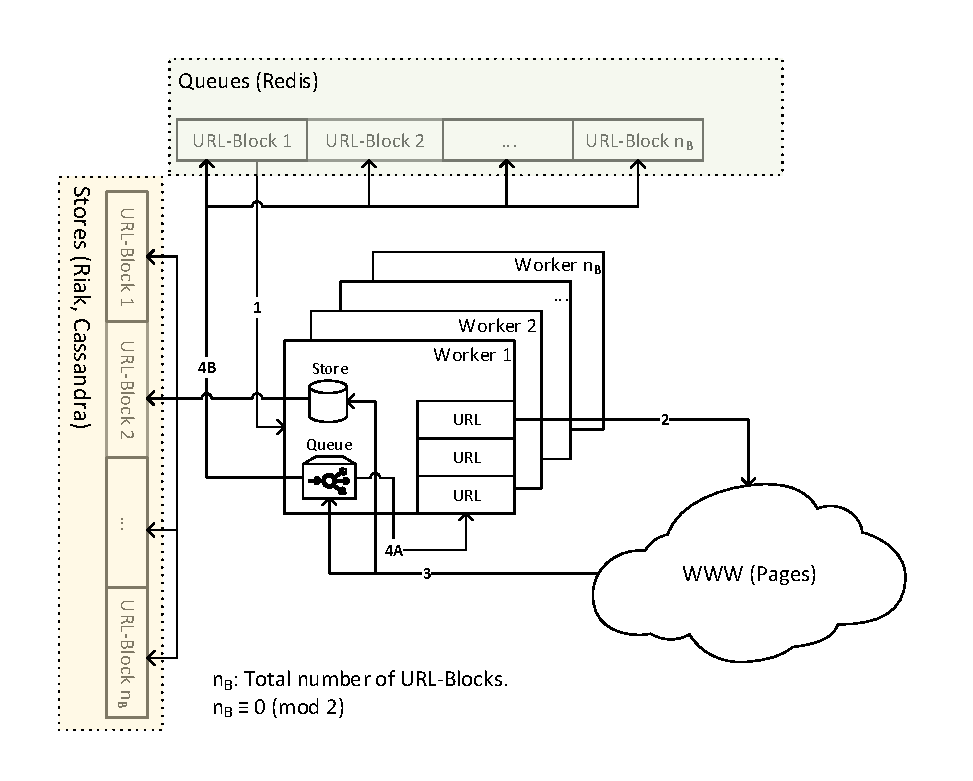
\includegraphics[width=1\textwidth]{Figures/system_overview.pdf}
\caption{Crawl.js - System Overview}
\label{system_overview}
\end{figure}

\section{Mapper}
\label{mapper}
The mapper is not a physical component in the system like the \emph{Queue}, the \emph{Worker} or the \emph{Store}. It is a algorithm allowing each component at any time to map an URL to an identifier. This identifier is then primarily used to determine the responsible \emph{Queue} or \emph{Store} for that URL.
This ability of being able to compute an identifier for a URL \emph{independently} is key to the whole system architecture. This ability is what makes the system decentralized. We don't have to ask a central component with manager like capabilities. We can compute the identifier ourself. Basically it identifies a virtual block within the URL space (all URLs). Every URL belongs to one and only one virtual block and each block is:
\begin{itemize}
  \item Mutual exclusive - Each block belongs to one and one worker only.
  \item Equally sized - From block to block the number of URLs should roughly be the same.
\end{itemize}

In other words the mapper is responsible to \emph{split} the work. In Crawl.js the mapper is nothing more than a function implemented as a separate module. Each component that needs to be able to map an URL to an identifier just include the module. The algorithm used is rather simple and illustrated below:
\begin{algorithmic}[0]
\Function{Map}{$url$}\Comment{Map the URL to an identifier}
\State $host \gets url.host$\Comment{Only the host part ex. www.unine.ch}
\State $hash \gets \textbf{hash}(host)$\Comment{Hash the host part}
\State $id \gets hash \bmod n$\Comment{id $\in \{0,1,..n\}$, n:total number of virtual blocks}
\State \textbf{return} $id$
\EndFunction
\end{algorithmic}

So the idea is to hash the host part of the URL modulo the total number of blocks we want. The modulo number (total number of blocks) must be shared among every component using the mapper in the system.
To achieve this shared knowledge we can use a \emph{static} or a \emph{dynamic} approach. Using the static one is much simpler and achievable through simple configuration values. The key about the \emph{static} approach is that the number doesn't change during runtime. If we want to change the configuration, we have to shutdown all workers, reconfigure them and restart. Using the \emph{dynamic} approach would allow us to change the value while all workers continue to run. They would simply start mapping URLs to new identifiers as soon as we change the value. It is obvious that for the dynamic approach some sort of communication between the mappers is needed to interchange the newly assigned value of "total number of virtual url blocks".

TODO: Dynamic approach

\subsection{Politeness}
To start, what does it mean for a crawler to be polite. There are different aspects of politeness like the robots exclusion protocol (discussed in \ref{worker}) that we don't want to discuss here. We want to discuss how often a crawler should access a server within a time frame. It is not especially the number (ex. once every 30 seconds) that is important but the fact that we need to be able to limit/control this number.

In order to do that we hash only the host part of the URL in our mapping function. Doing so guarantees that there is always only one worker responsible for one host. Having this situation allows us now to control this aspect of politeness.
During our first test runs we accidentally hashed the whole URL. This resulted in an uncontrollable situation because multiple workers were fetching the same host simultaneously.

\section{Queues}
Queues play a central role in the Crawl.js system. There are \emph{local} queues and \emph{remote} queues. Each worker keeps a local, in-memory queue during his crawl for various reasons discussed in section \ref{queues_local} and each worker \emph{consumes} URLs from a remote queue. A remote queue represents one virtual URL block (as discussed in section \ref{mapper}). But, before we start with the details we state more precisely the term queue used in Crawl.js.

\subsection{Queue}
First a few words about how we use the word \emph{Queue} within this document. Strictly and technically speaking it is \emph{more} than a queue. A basic queue has the following operations:
\begin{itemize}
  \item enqueue
  \item dequeue
\end{itemize}

New items are enqueued at the bottom of the list and existing items are dequeued from the top. In terms of URLs this could work. But, what if we want to prioritize the URLs in the queue in some way. Of course we could enqueue URLs in the order we want them prioritized but this is rather inconvenient and does not work for existing URLs in the queue. We want to be able to re-prioritize (remove/change) existing URLs in the queue. And as mentioned in \cite{hp_crawler} fetching URLs in the order they were enqueued is a bad idea because of second-level locality in the links.

Therefore in Crawl.js a queue is a \emph{sorted set}. With sorted sets we can achieve whatever order we like. We can simulate a queue with it (thats why we still call it queue), use a pure random approach (set) or use custom algorithms to compute the order in the queues (re-visit policies).

\subsection{Consuming \& Producing}
The \emph{consumer} is the worker. Only one worker. So, the worker needs to know from which remote queue to consume from. This information is given as startup parameter. The parameter is not only the identifier of the queue but the identifier of the virtual URL block this worker is responsible for. We discussed the ability of every worker being able to map an URL to an id in section \ref{mapper}. With the help of this additional parameter the worker is now able to decide if he is responsible for a given URL (compare the ids). If he is the URL is added to the \emph{local} queue. If he is not the URL is added to appropriate \emph{remote} queue. Doing so makes the worker also a \emph{producer}. Obviously because there are multiple workers acting the same, we have a multiple producer situation for a single remote queue. 

\subsection{Local Queue (in-memory)}
\label{queues_local}
As the title describes it, from the worker's point of view it is a local and in-memory queue. The reason why every worker has a local queue is twofold:
\begin{itemize}
  \item We want the worker to be autonomous for a certain time. Therefore he needs a place to put the newly found URLs (during his crawl).
  \item Additionally we don't want to fetch the same URL twice (during one crawl of one worker). Therefore the local queue is the first filter used to eliminate duplicated URLs. Because the Queue is implemented as a sorted set, checking for the existence of an URL is easy an achievable in the complexity of O(1).
\end{itemize}

One thing to note is that the state of this local queue is in memory only. This means that when the worker crashes this state is lost. So we need to find a trade off between autonomy and fault tolerance. We want the worker to be autonomous (no inter communication) as much as possible, but on the other side we don't want to loose to much information if a worker crashes. Currently this trade off is adjustable with the help of a configuration value that limits the queue in size. Once this limit is reached, the worker does not put any new URLs in the local queue but dispatches them to the \emph{remote} one. This allows him to empty his queue and finish his crawl. An additional idea would be to limit a crawl in terms of time, but this is not implemented yet.

\subsection{Remote Queue}
\label{queues_remote}
As mentioned in the introduction of this section one worker is responsible to empty his queue and all other workers are able to fill it. The state of all remote queues represents the whole system state. URLs on the top of those queues are going to be fetched next and URLs at the bottom have just been fetched successfully. It is obvious that this state is important and need to be persisted. 


\subsection{Remote Queue implementation (Redis.io)}
In Crawl.js remote queues are implemented with Redis\footnote{Redis - \url{http://www.redis.io}}. We use one sorted set for one remote queue. Luckily the sorted set from Redis gives us all the atomic operations we need. Redis uses the notion of score to sort the elements in the set. With the help of this score value we can not only sort the elements within the queue, but we can also store state information with it (ex. score > 0 := FETCHED, score < 0 := FETCH). Each element in the sorted set is a tuple (member,score) where the member is an URL in our case. How the worker uses the score together with the available commands is described below. Low (even negative) score values represent URLs that are going to be fetched next.

\begin{enumerate}
  \item \textbf{ZRANGEBYSCORE}\footnote{\url{http://redis.io/commands/zrangebyscore}} (single consumer) - get next URLs that need to be fetched. Note that the elements in the queue are not removed yet.
  \item \textbf{ZINCRBY} (multiple producers) - decrement the score of URL by a constant value. This happens when workers dispatch extracted URLs. It makes the entry move up the queue.
  \item \textbf{ZADD} (single producer) - As soon as an URL is fetched successfully we set the score to the current time stamp. This makes the entry move to the bottom of the queue.
\end{enumerate}

This is maybe not the best approach of how to prioritize URLs within the remote queues, but it is was simple to implement and allowed us to run first tests. The important thing to note here is that we have set a base with sorted sets that allows us to easily try out new approaches. As an example we could introduce an independent component in the system that takes care of computing the order of our queues based on some algorithms. (ex. Page rank).

\subsection{Memory usage (Redis.io)}

\section{Stores}
Ola store
\subsection{Implementation (Riak)}

\section{Worker (a crawl.js instance)}
\label{worker}
A worker is autonomous and responsible for one URL-Block. Why autonomous? Because a worker can fetch pages, store them and extract new URLs out of it. Newly found URLs are assigned (\emph{Mapper}) to their URL-Block and dispatched automatically. All this happens without any interaction to other components in the system. This keeps the number of inter-communication messages very low.

One worker for one URL-Block. This is true for consuming URLs but obviously we have multiple URL producers. Namely each worker in the system is a candidate for producing new URLs because each one is able to assign and dispatch newly found URLs independly. So we have one consumer and multiple producers whithin one URL-Block (queue).
\subsection{States}
Dummy
\subsection{Software Architecture}
Dummy
\subsection{Configuration}
Dummy
\subsection{github}
Dummy
\subsection{Performance}
Dummy
\subsection{Storage}
Dummy
\subsection{Details - (Url-normalization, ..)}

